% GNUPLOT: LaTeX picture with Postscript
\begingroup
  \makeatletter
  \providecommand\color[2][]{%
    \GenericError{(gnuplot) \space\space\space\@spaces}{%
      Package color not loaded in conjunction with
      terminal option `colourtext'%
    }{See the gnuplot documentation for explanation.%
    }{Either use 'blacktext' in gnuplot or load the package
      color.sty in LaTeX.}%
    \renewcommand\color[2][]{}%
  }%
  \providecommand\includegraphics[2][]{%
    \GenericError{(gnuplot) \space\space\space\@spaces}{%
      Package graphicx or graphics not loaded%
    }{See the gnuplot documentation for explanation.%
    }{The gnuplot epslatex terminal needs graphicx.sty or graphics.sty.}%
    \renewcommand\includegraphics[2][]{}%
  }%
  \providecommand\rotatebox[2]{#2}%
  \@ifundefined{ifGPcolor}{%
    \newif\ifGPcolor
    \GPcolortrue
  }{}%
  \@ifundefined{ifGPblacktext}{%
    \newif\ifGPblacktext
    \GPblacktexttrue
  }{}%
  % define a \g@addto@macro without @ in the name:
  \let\gplgaddtomacro\g@addto@macro
  % define empty templates for all commands taking text:
  \gdef\gplbacktext{}%
  \gdef\gplfronttext{}%
  \makeatother
  \ifGPblacktext
    % no textcolor at all
    \def\colorrgb#1{}%
    \def\colorgray#1{}%
  \else
    % gray or color?
    \ifGPcolor
      \def\colorrgb#1{\color[rgb]{#1}}%
      \def\colorgray#1{\color[gray]{#1}}%
      \expandafter\def\csname LTw\endcsname{\color{white}}%
      \expandafter\def\csname LTb\endcsname{\color{black}}%
      \expandafter\def\csname LTa\endcsname{\color{black}}%
      \expandafter\def\csname LT0\endcsname{\color[rgb]{1,0,0}}%
      \expandafter\def\csname LT1\endcsname{\color[rgb]{0,1,0}}%
      \expandafter\def\csname LT2\endcsname{\color[rgb]{0,0,1}}%
      \expandafter\def\csname LT3\endcsname{\color[rgb]{1,0,1}}%
      \expandafter\def\csname LT4\endcsname{\color[rgb]{0,1,1}}%
      \expandafter\def\csname LT5\endcsname{\color[rgb]{1,1,0}}%
      \expandafter\def\csname LT6\endcsname{\color[rgb]{0,0,0}}%
      \expandafter\def\csname LT7\endcsname{\color[rgb]{1,0.3,0}}%
      \expandafter\def\csname LT8\endcsname{\color[rgb]{0.5,0.5,0.5}}%
    \else
      % gray
      \def\colorrgb#1{\color{black}}%
      \def\colorgray#1{\color[gray]{#1}}%
      \expandafter\def\csname LTw\endcsname{\color{white}}%
      \expandafter\def\csname LTb\endcsname{\color{black}}%
      \expandafter\def\csname LTa\endcsname{\color{black}}%
      \expandafter\def\csname LT0\endcsname{\color{black}}%
      \expandafter\def\csname LT1\endcsname{\color{black}}%
      \expandafter\def\csname LT2\endcsname{\color{black}}%
      \expandafter\def\csname LT3\endcsname{\color{black}}%
      \expandafter\def\csname LT4\endcsname{\color{black}}%
      \expandafter\def\csname LT5\endcsname{\color{black}}%
      \expandafter\def\csname LT6\endcsname{\color{black}}%
      \expandafter\def\csname LT7\endcsname{\color{black}}%
      \expandafter\def\csname LT8\endcsname{\color{black}}%
    \fi
  \fi
    \setlength{\unitlength}{0.0500bp}%
    \ifx\gptboxheight\undefined%
      \newlength{\gptboxheight}%
      \newlength{\gptboxwidth}%
      \newsavebox{\gptboxtext}%
    \fi%
    \setlength{\fboxrule}{0.5pt}%
    \setlength{\fboxsep}{1pt}%
    \definecolor{tbcol}{rgb}{1,1,1}%
\begin{picture}(4520.00,4240.00)%
    \gplgaddtomacro\gplbacktext{%
    }%
    \gplgaddtomacro\gplfronttext{%
      \csname LTb\endcsname%%
      \put(577,2476){\makebox(0,0)[r]{\strut{}$-160$}}%
      \csname LTb\endcsname%%
      \put(577,2662){\makebox(0,0)[r]{\strut{}$-120$}}%
      \csname LTb\endcsname%%
      \put(577,2847){\makebox(0,0)[r]{\strut{}$-80$}}%
      \csname LTb\endcsname%%
      \put(577,3032){\makebox(0,0)[r]{\strut{}$-40$}}%
      \csname LTb\endcsname%%
      \put(577,3217){\makebox(0,0)[r]{\strut{}$0$}}%
      \csname LTb\endcsname%%
      \put(577,3402){\makebox(0,0)[r]{\strut{}$40$}}%
      \csname LTb\endcsname%%
      \put(577,3588){\makebox(0,0)[r]{\strut{}$80$}}%
      \csname LTb\endcsname%%
      \put(577,3773){\makebox(0,0)[r]{\strut{}$120$}}%
      \csname LTb\endcsname%%
      \put(577,3958){\makebox(0,0)[r]{\strut{}$160$}}%
      \csname LTb\endcsname%%
      \put(675,2208){\makebox(0,0){\strut{}}}%
      \csname LTb\endcsname%%
      \put(952,2208){\makebox(0,0){\strut{}}}%
      \csname LTb\endcsname%%
      \put(1230,2208){\makebox(0,0){\strut{}}}%
      \csname LTb\endcsname%%
      \put(1508,2208){\makebox(0,0){\strut{}}}%
      \csname LTb\endcsname%%
      \put(1786,2208){\makebox(0,0){\strut{}}}%
      \csname LTb\endcsname%%
      \put(2064,2208){\makebox(0,0){\strut{}}}%
      \csname LTb\endcsname%%
      \put(2341,2208){\makebox(0,0){\strut{}}}%
      \csname LTb\endcsname%%
      \put(219,3217){\rotatebox{-270.00}{\makebox(0,0){\normalsize $\Psi$}}}%
      \csname LTb\endcsname%%
      \put(1333,3314){\rotatebox{-63.00}{\makebox(0,0){\strut{}\textcolor{black}{\footnotesize 500}}}}%
      \csname LTb\endcsname%%
      \put(1669,3265){\rotatebox{130.00}{\makebox(0,0){\strut{}\textcolor{black}{\footnotesize 400}}}}%
      \csname LTb\endcsname%%
      \put(1382,3126){\rotatebox{-46.00}{\makebox(0,0){\strut{}\textcolor{black}{\footnotesize 400}}}}%
      \csname LTb\endcsname%%
      \put(1364,3560){\rotatebox{157.00}{\makebox(0,0){\strut{}\textcolor{black}{\footnotesize 300}}}}%
      \csname LTb\endcsname%%
      \put(1445,2980){\rotatebox{-39.00}{\makebox(0,0){\strut{}\textcolor{black}{\footnotesize 300}}}}%
      \csname LTb\endcsname%%
      \put(1874,3182){\rotatebox{115.00}{\makebox(0,0){\strut{}\textcolor{black}{\footnotesize 200}}}}%
      \csname LTb\endcsname%%
      \put(1067,3689){\rotatebox{-140.00}{\makebox(0,0){\strut{}\textcolor{black}{\footnotesize 200}}}}%
      \csname LTb\endcsname%%
      \put(1511,2860){\rotatebox{-24.00}{\makebox(0,0){\strut{}\textcolor{black}{\footnotesize 200}}}}%
      \csname LTb\endcsname%%
      \put(1067,3034){\rotatebox{39.00}{\makebox(0,0){\strut{}\textcolor{black}{\footnotesize 100}}}}%
      \csname LTb\endcsname%%
      \put(1040,3897){\rotatebox{44.00}{\makebox(0,0){\strut{}\textcolor{black}{\footnotesize 100}}}}%
      \csname LTb\endcsname%%
      \put(1781,3827){\rotatebox{62.00}{\makebox(0,0){\strut{}\textcolor{black}{\footnotesize 100}}}}%
      \csname LTb\endcsname%%
      \put(1934,3224){\rotatebox{-73.00}{\makebox(0,0){\strut{}\textcolor{black}{\footnotesize 100}}}}%
      \csname LTb\endcsname%%
      \put(955,2721){\rotatebox{-33.00}{\makebox(0,0){\strut{}\textcolor{black}{\footnotesize 100}}}}%
      \csname LTb\endcsname%%
      \put(1845,2580){\rotatebox{-44.00}{\makebox(0,0){\strut{}\textcolor{black}{\footnotesize 100}}}}%
      \csname LTb\endcsname%%
      \put(729,3392){\rotatebox{-104.00}{\makebox(0,0){\strut{}\textcolor{black}{\footnotesize 50}}}}%
      \csname LTb\endcsname%%
      \put(1442,3911){\rotatebox{158.00}{\makebox(0,0){\strut{}\textcolor{black}{\footnotesize 50}}}}%
      \csname LTb\endcsname%%
      \put(1262,2468){\rotatebox{-72.00}{\makebox(0,0){\strut{}\textcolor{black}{\footnotesize 50}}}}%
      \csname LTb\endcsname%%
      \put(2033,3352){\rotatebox{-139.00}{\makebox(0,0){\strut{}\textcolor{black}{\footnotesize 50}}}}%
      \csname LTb\endcsname%%
      \put(1508,4174){\makebox(0,0){\strut{}Conformational Energy (meV)}}%
    }%
    \gplgaddtomacro\gplbacktext{%
    }%
    \gplgaddtomacro\gplfronttext{%
      \csname LTb\endcsname%%
      \put(2512,2476){\makebox(0,0)[r]{\strut{}}}%
      \csname LTb\endcsname%%
      \put(2512,2662){\makebox(0,0)[r]{\strut{}}}%
      \csname LTb\endcsname%%
      \put(2512,2847){\makebox(0,0)[r]{\strut{}}}%
      \csname LTb\endcsname%%
      \put(2512,3032){\makebox(0,0)[r]{\strut{}}}%
      \csname LTb\endcsname%%
      \put(2512,3217){\makebox(0,0)[r]{\strut{}}}%
      \csname LTb\endcsname%%
      \put(2512,3402){\makebox(0,0)[r]{\strut{}}}%
      \csname LTb\endcsname%%
      \put(2512,3588){\makebox(0,0)[r]{\strut{}}}%
      \csname LTb\endcsname%%
      \put(2512,3773){\makebox(0,0)[r]{\strut{}}}%
      \csname LTb\endcsname%%
      \put(2512,3958){\makebox(0,0)[r]{\strut{}}}%
      \csname LTb\endcsname%%
      \put(2610,2208){\makebox(0,0){\strut{}}}%
      \csname LTb\endcsname%%
      \put(2887,2208){\makebox(0,0){\strut{}}}%
      \csname LTb\endcsname%%
      \put(3165,2208){\makebox(0,0){\strut{}}}%
      \csname LTb\endcsname%%
      \put(3443,2208){\makebox(0,0){\strut{}}}%
      \csname LTb\endcsname%%
      \put(3721,2208){\makebox(0,0){\strut{}}}%
      \csname LTb\endcsname%%
      \put(3999,2208){\makebox(0,0){\strut{}}}%
      \csname LTb\endcsname%%
      \put(4276,2208){\makebox(0,0){\strut{}}}%
      \csname LTb\endcsname%%
      \put(3672,2602){\rotatebox{43.00}{\makebox(0,0){\strut{}\textcolor{black}{\footnotesize 3.0}}}}%
      \csname LTb\endcsname%%
      \put(3573,3160){\rotatebox{129.00}{\makebox(0,0){\strut{}\textcolor{black}{\footnotesize 2.5}}}}%
      \csname LTb\endcsname%%
      \put(2921,3850){\rotatebox{-72.00}{\makebox(0,0){\strut{}\textcolor{black}{\footnotesize 2.5}}}}%
      \csname LTb\endcsname%%
      \put(3489,3962){\makebox(0,0){\strut{}\textcolor{black}{\footnotesize 2.5}}}%
      \csname LTb\endcsname%%
      \put(3012,2474){\rotatebox{40.00}{\makebox(0,0){\strut{}\textcolor{black}{\footnotesize 2.5}}}}%
      \csname LTb\endcsname%%
      \put(3590,2695){\rotatebox{42.00}{\makebox(0,0){\strut{}\textcolor{black}{\footnotesize 2.5}}}}%
      \csname LTb\endcsname%%
      \put(4142,2922){\rotatebox{-22.00}{\makebox(0,0){\strut{}\textcolor{black}{\footnotesize 2.5}}}}%
      \csname LTb\endcsname%%
      \put(2829,3967){\rotatebox{-108.00}{\makebox(0,0){\strut{}\textcolor{black}{\footnotesize 2.0}}}}%
      \csname LTb\endcsname%%
      \put(3037,3599){\rotatebox{-4.00}{\makebox(0,0){\strut{}\textcolor{black}{\footnotesize 2.0}}}}%
      \csname LTb\endcsname%%
      \put(3598,3847){\rotatebox{-5.00}{\makebox(0,0){\strut{}\textcolor{black}{\footnotesize 2.0}}}}%
      \csname LTb\endcsname%%
      \put(3338,2628){\rotatebox{24.00}{\makebox(0,0){\strut{}\textcolor{black}{\footnotesize 2.0}}}}%
      \csname LTb\endcsname%%
      \put(3422,3043){\rotatebox{145.00}{\makebox(0,0){\strut{}\textcolor{black}{\footnotesize 2.0}}}}%
      \csname LTb\endcsname%%
      \put(3330,3424){\rotatebox{-23.00}{\makebox(0,0){\strut{}\textcolor{black}{\footnotesize 2.0}}}}%
      \csname LTb\endcsname%%
      \put(3824,3097){\rotatebox{-19.00}{\makebox(0,0){\strut{}\textcolor{black}{\footnotesize 2.0}}}}%
      \csname LTb\endcsname%%
      \put(2729,3230){\rotatebox{50.00}{\makebox(0,0){\strut{}\textcolor{black}{\footnotesize 1.5}}}}%
      \csname LTb\endcsname%%
      \put(3196,3130){\rotatebox{-50.00}{\makebox(0,0){\strut{}\textcolor{black}{\footnotesize 1.5}}}}%
      \csname LTb\endcsname%%
      \put(3229,2704){\rotatebox{-173.00}{\makebox(0,0){\strut{}\textcolor{black}{\footnotesize 1.5}}}}%
      \csname LTb\endcsname%%
      \put(3875,3774){\rotatebox{-155.00}{\makebox(0,0){\strut{}\textcolor{black}{\footnotesize 1.5}}}}%
      \csname LTb\endcsname%%
      \put(3414,3514){\rotatebox{-36.00}{\makebox(0,0){\strut{}\textcolor{black}{\footnotesize 1.5}}}}%
      \csname LTb\endcsname%%
      \put(3950,3260){\rotatebox{16.00}{\makebox(0,0){\strut{}\textcolor{black}{\footnotesize 1.5}}}}%
      \csname LTb\endcsname%%
      \put(2673,2560){\rotatebox{75.00}{\makebox(0,0){\strut{}\textcolor{black}{\footnotesize 1.0}}}}%
      \csname LTb\endcsname%%
      \put(2878,3156){\rotatebox{14.00}{\makebox(0,0){\strut{}\textcolor{black}{\footnotesize 1.0}}}}%
      \csname LTb\endcsname%%
      \put(3070,2775){\rotatebox{-156.00}{\makebox(0,0){\strut{}\textcolor{black}{\footnotesize 1.0}}}}%
      \csname LTb\endcsname%%
      \put(3841,3666){\rotatebox{-158.00}{\makebox(0,0){\strut{}\textcolor{black}{\footnotesize 1.0}}}}%
      \csname LTb\endcsname%%
      \put(3958,3372){\rotatebox{11.00}{\makebox(0,0){\strut{}\textcolor{black}{\footnotesize 1.0}}}}%
      \csname LTb\endcsname%%
      \put(3022,2970){\rotatebox{116.00}{\makebox(0,0){\strut{}\textcolor{black}{\footnotesize 0.5}}}}%
      \csname LTb\endcsname%%
      \put(3443,4174){\makebox(0,0){Dipole Strength (Debye)}}%
    }%
    \gplgaddtomacro\gplbacktext{%
    }%
    \gplgaddtomacro\gplfronttext{%
      \csname LTb\endcsname%%
      \put(577,556){\makebox(0,0)[r]{\strut{}$-160$}}%
      \csname LTb\endcsname%%
      \put(577,742){\makebox(0,0)[r]{\strut{}$-120$}}%
      \csname LTb\endcsname%%
      \put(577,927){\makebox(0,0)[r]{\strut{}$-80$}}%
      \csname LTb\endcsname%%
      \put(577,1112){\makebox(0,0)[r]{\strut{}$-40$}}%
      \csname LTb\endcsname%%
      \put(577,1297){\makebox(0,0)[r]{\strut{}$0$}}%
      \csname LTb\endcsname%%
      \put(577,1482){\makebox(0,0)[r]{\strut{}$40$}}%
      \csname LTb\endcsname%%
      \put(577,1668){\makebox(0,0)[r]{\strut{}$80$}}%
      \csname LTb\endcsname%%
      \put(577,1853){\makebox(0,0)[r]{\strut{}$120$}}%
      \csname LTb\endcsname%%
      \put(577,2038){\makebox(0,0)[r]{\strut{}$160$}}%
      \csname LTb\endcsname%%
      \put(767,288){\makebox(0,0){\strut{}$-160$}}%
      \csname LTb\endcsname%%
      \put(1138,288){\makebox(0,0){\strut{}$-80$}}%
      \csname LTb\endcsname%%
      \put(1508,288){\makebox(0,0){\strut{}$0$}}%
      \csname LTb\endcsname%%
      \put(1878,288){\makebox(0,0){\strut{}$80$}}%
      \csname LTb\endcsname%%
      \put(2249,288){\makebox(0,0){\strut{}$160$}}%
      \csname LTb\endcsname%%
      \put(219,1297){\rotatebox{-270.00}{\makebox(0,0){\normalsize $\Psi$}}}%
      \csname LTb\endcsname%%
      \put(1508,24){\makebox(0,0){\normalsize $\Phi$}}%
      \csname LTb\endcsname%%
      \put(1451,1423){\rotatebox{148.00}{\makebox(0,0){\strut{}\textcolor{black}{\footnotesize 1.3}}}}%
      \csname LTb\endcsname%%
      \put(1348,1228){\rotatebox{-45.00}{\makebox(0,0){\strut{}\textcolor{black}{\footnotesize 1.4}}}}%
      \csname LTb\endcsname%%
      \put(1683,1423){\rotatebox{143.00}{\makebox(0,0){\strut{}\textcolor{black}{\footnotesize 1.5}}}}%
      \csname LTb\endcsname%%
      \put(1488,1019){\rotatebox{-45.00}{\makebox(0,0){\strut{}\textcolor{black}{\footnotesize 1.5}}}}%
      \csname LTb\endcsname%%
      \put(1285,1726){\rotatebox{45.00}{\makebox(0,0){\strut{}\textcolor{black}{\footnotesize 1.6}}}}%
      \csname LTb\endcsname%%
      \put(1904,1061){\rotatebox{48.00}{\makebox(0,0){\strut{}\textcolor{black}{\footnotesize 1.6}}}}%
      \csname LTb\endcsname%%
      \put(895,1726){\rotatebox{-34.00}{\makebox(0,0){\strut{}\textcolor{black}{\footnotesize 1.7}}}}%
      \csname LTb\endcsname%%
      \put(1189,733){\rotatebox{112.00}{\makebox(0,0){\strut{}\textcolor{black}{\footnotesize 1.7}}}}%
      \csname LTb\endcsname%%
      \put(1988,2032){\rotatebox{-135.00}{\makebox(0,0){\strut{}\textcolor{black}{\footnotesize 1.7}}}}%
      \csname LTb\endcsname%%
      \put(1937,590){\rotatebox{-25.00}{\makebox(0,0){\strut{}\textcolor{black}{\footnotesize 1.7}}}}%
      \csname LTb\endcsname%%
      \put(1508,2254){\makebox(0,0){VBA EA (eV)}}%
    }%
    \gplgaddtomacro\gplbacktext{%
    }%
    \gplgaddtomacro\gplfronttext{%
      \csname LTb\endcsname%%
      \put(2512,556){\makebox(0,0)[r]{\strut{}}}%
      \csname LTb\endcsname%%
      \put(2512,742){\makebox(0,0)[r]{\strut{}}}%
      \csname LTb\endcsname%%
      \put(2512,927){\makebox(0,0)[r]{\strut{}}}%
      \csname LTb\endcsname%%
      \put(2512,1112){\makebox(0,0)[r]{\strut{}}}%
      \csname LTb\endcsname%%
      \put(2512,1297){\makebox(0,0)[r]{\strut{}}}%
      \csname LTb\endcsname%%
      \put(2512,1482){\makebox(0,0)[r]{\strut{}}}%
      \csname LTb\endcsname%%
      \put(2512,1668){\makebox(0,0)[r]{\strut{}}}%
      \csname LTb\endcsname%%
      \put(2512,1853){\makebox(0,0)[r]{\strut{}}}%
      \csname LTb\endcsname%%
      \put(2512,2038){\makebox(0,0)[r]{\strut{}}}%
      \csname LTb\endcsname%%
      \put(2702,288){\makebox(0,0){\strut{}$-160$}}%
      \csname LTb\endcsname%%
      \put(3073,288){\makebox(0,0){\strut{}$-80$}}%
      \csname LTb\endcsname%%
      \put(3443,288){\makebox(0,0){\strut{}$0$}}%
      \csname LTb\endcsname%%
      \put(3813,288){\makebox(0,0){\strut{}$80$}}%
      \csname LTb\endcsname%%
      \put(4184,288){\makebox(0,0){\strut{}$160$}}%
      \csname LTb\endcsname%%
      \put(3443,24){\makebox(0,0){\normalsize $\Phi$}}%
      \csname LTb\endcsname%%
      \put(3576,1120){\rotatebox{-34.00}{\makebox(0,0){\strut{}\textcolor{black}{\footnotesize 9}}}}%
      \csname LTb\endcsname%%
      \put(3771,558){\rotatebox{-22.00}{\makebox(0,0){\strut{}\textcolor{black}{\footnotesize 9}}}}%
      \csname LTb\endcsname%%
      \put(3637,769){\rotatebox{69.00}{\makebox(0,0){\strut{}\textcolor{black}{\footnotesize 6}}}}%
      \csname LTb\endcsname%%
      \put(3562,1306){\rotatebox{-38.00}{\makebox(0,0){\strut{}\textcolor{black}{\footnotesize 6}}}}%
      \csname LTb\endcsname%%
      \put(3940,515){\rotatebox{-151.00}{\makebox(0,0){\strut{}\textcolor{black}{\footnotesize 6}}}}%
      \csname LTb\endcsname%%
      \put(3188,1844){\rotatebox{39.00}{\makebox(0,0){\strut{}\textcolor{black}{\footnotesize 3}}}}%
      \csname LTb\endcsname%%
      \put(3603,875){\rotatebox{70.00}{\makebox(0,0){\strut{}\textcolor{black}{\footnotesize 3}}}}%
      \csname LTb\endcsname%%
      \put(3569,1349){\rotatebox{-39.00}{\makebox(0,0){\strut{}\textcolor{black}{\footnotesize 3}}}}%
      \csname LTb\endcsname%%
      \put(4057,532){\rotatebox{-131.00}{\makebox(0,0){\strut{}\textcolor{black}{\footnotesize 3}}}}%
      \csname LTb\endcsname%%
      \put(3899,2080){\rotatebox{24.00}{\makebox(0,0){\strut{}\textcolor{black}{\footnotesize 3}}}}%
      \csname LTb\endcsname%%
      \put(3352,2013){\rotatebox{91.00}{\makebox(0,0){\strut{}\textcolor{black}{\footnotesize 1}}}}%
      \csname LTb\endcsname%%
      \put(3956,2066){\rotatebox{28.00}{\makebox(0,0){\strut{}\textcolor{black}{\footnotesize 1}}}}%
      \csname LTb\endcsname%%
      \put(3467,1036){\rotatebox{128.00}{\makebox(0,0){\strut{}\textcolor{black}{\footnotesize 1}}}}%
      \csname LTb\endcsname%%
      \put(3612,1356){\rotatebox{-34.00}{\makebox(0,0){\strut{}\textcolor{black}{\footnotesize 1}}}}%
      \csname LTb\endcsname%%
      \put(4116,548){\rotatebox{-116.00}{\makebox(0,0){\strut{}\textcolor{black}{\footnotesize 1}}}}%
      \csname LTb\endcsname%%
      \put(2860,1547){\makebox(0,0){\strut{}\textcolor{black}{\normalsize \textbf{C}}}}%
      \csname LTb\endcsname%%
      \put(4026,1247){\makebox(0,0){\strut{}\textcolor{black}{\normalsize \textbf{B}}}}%
      \csname LTb\endcsname%%
      \put(3243,1130){\makebox(0,0){\strut{}\textcolor{black}{\normalsize \textbf{A}}}}%
      \csname LTb\endcsname%%
      \put(3443,2254){\makebox(0,0){DBA EA (meV)}}%
    }%
    \gplbacktext
    \put(0,0){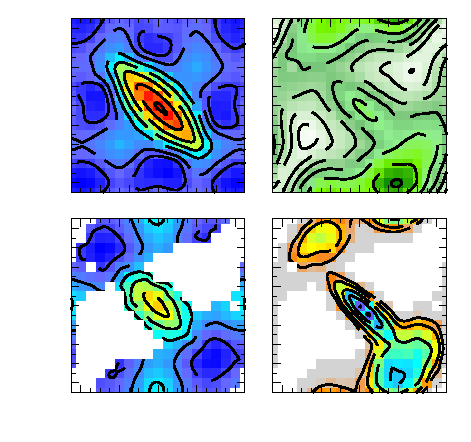
\includegraphics[width={226.00bp},height={212.00bp}]{Figs/Q1_maps}}%
    \gplfronttext
  \end{picture}%
\endgroup
